% !TEX encoding = UTF-8
% !TEX program = xelatex

\documentclass[aspectratio=169, 10pt, fontset=fandol]{ctexbeamer}

\usetheme{Boadilla}
\usecolortheme{default}
\usefonttheme{professionalfonts}

\usepackage{amsmath, amssymb, mathtools}
\usepackage{booktabs}
\usepackage{graphicx}
\usepackage{tabularx}
\usepackage{array}
\usepackage{unicode-math}
\usepackage{tikz}

\graphicspath{{figures/}}

\setmathfont{XITSMath-Regular.otf}
\setbeamertemplate{navigation symbols}{}
\setbeamertemplate{caption}[numbered]
\setbeamertemplate{footline}[frame number]

\definecolor{ustcblue}{RGB}{0,82,155}
\definecolor{ustcred}{RGB}{178,34,52}
\setbeamercolor{structure}{fg=ustcblue}
\setbeamercolor{title}{fg=ustcblue}
\setbeamercolor{frametitle}{fg=ustcblue,bg=white}
\setbeamercolor{section label}{fg=gray!70}
\setbeamercolor{block title}{fg=white,bg=ustcblue}
\setbeamercolor{block body}{bg=ustcblue!4}
\setbeamercolor{alerted text}{fg=ustcred}

\setbeamertemplate{frametitle}{%
  \vspace{0.18cm}%
  \nointerlineskip
  \begin{beamercolorbox}[wd=\textwidth,sep=0pt]{frametitle}
    \usebeamerfont{frametitle}\insertframetitle%
    \hfill
    {\usebeamercolor[fg]{section label}\scriptsize\insertsectionhead}
  \end{beamercolorbox}%
  \vspace{0.08cm}
  {\color{ustcblue!55}\rule{\textwidth}{0.45pt}}%
}

\newcommand\dif{\mathop{}\!\mathrm{d}}
\newcommand\T{\operatorname{T}}
\newcommand\R{\mathbb{R}}
\newcommand\bsde{BSDE}
\newcommand\rfm{RFM}
\newcommand\mc{MC}

\title[随机特征方法求解高维抛物型方程]{随机特征方法求解高维抛物型方程}
\subtitle{本科毕业论文答辩}
\author[刘行]{刘行}
\institute[中国科学技术大学]{中国科学技术大学 \quad 少年班学院\\信息与计算科学}
\date{\today}

% Keep school marks only on the title and closing pages, not on every slide.

\AtBeginSection[]{
  \begin{frame}[plain,noframenumbering]
    \begin{center}
      \vspace{1.2cm}
      {\Large 第 \insertsectionnumber 部分}

      \vspace{0.4cm}
      {\huge\bfseries\color{ustcblue}\insertsectionhead}
    \end{center}
  \end{frame}
}

\begin{document}

\begin{frame}[plain]
  \begin{tikzpicture}[remember picture,overlay]
    \node[anchor=north east, xshift=-0.55cm, yshift=-0.35cm]
      at (current page.north east)
      {
\includegraphics[height=1.05cm]{ustc-badge}};
    \node[anchor=north west, xshift=0.55cm, yshift=-0.42cm]
      at (current page.north west)
      {
\includegraphics[height=0.78cm]{ustc-name}};
  \end{tikzpicture}

  \vspace{1.15cm}
  \begin{center}
    {\large 本科毕业论文答辩}

    \vspace{0.45cm}
    {\LARGE\bfseries\color{ustcblue} 随机特征方法求解高维抛物型方程}

    \vspace{0.45cm}
    {\large 刘行}

    \vspace{0.12cm}
    {\small 中国科学技术大学\\少年班学院 \quad 信息与计算科学}
  \end{center}

  \vspace{0.15cm}
  \begin{center}
    \small 指导教师: 陈景润教授 \qquad \today
  \end{center}
\end{frame}

\begin{frame}{汇报结构}
  \begin{enumerate}
    \item 问题背景: 高维抛物型 PDE 的初值计算.
    \item 方法: PDE-BSDE 转化与随机特征表示.
    \item 实现: C++/libtorch 中的线性与半线性求解器.
    \item 实验: 四个 $100$ 维算例, 参数敏感性与 Deep BSDE 对比.
    \item 总结: 方法特点, 局限与后续方向.
  \end{enumerate}
\end{frame}

\section{问题背景}

\begin{frame}{研究问题}
  \begin{columns}[T,onlytextwidth]
    \begin{column}{0.55\textwidth}
      \begin{block}{目标}
        对高维半线性抛物型终值问题, 计算给定初始点处的
        \begin{equation*}
          u(0,x_0).
        \end{equation*}
      \end{block}
      \vspace{0.2cm}
      统一方程写为
      \begin{equation*}
      \begin{aligned}
        &\partial_t u
        + \frac12 \operatorname{Tr}\!\bigl(\sigma\sigma^{\T}\nabla_x^2u\bigr)
        + \langle \mu,\nabla_x u\rangle \\
        &\quad + f\!\bigl(t,x,u,\sigma^{\T}\nabla_xu\bigr)=0,
        \qquad
        u(T,x)=g(x).
      \end{aligned}
      \end{equation*}
    \end{column}
    \begin{column}{0.40\textwidth}
      \begin{block}{困难}
        \begin{itemize}
          \item 网格型方法在 $d$ 维空间中规模随维度指数增长.
          \item 高维情形更适合从样本路径和函数逼近入手.
          \item 需要同时控制采样误差, 时间离散误差和函数逼近误差.
        \end{itemize}
      \end{block}
    \end{column}
  \end{columns}
\end{frame}

\section{方法框架}

\begin{frame}{方法主线: PDE 到 BSDE}
  令正向过程满足
  \begin{equation*}
    X_t=x_0+\int_0^t \mu(s,X_s)\,\dif s
        +\int_0^t \sigma(s,X_s)\,\dif W_s.
  \end{equation*}
  若
  \begin{equation*}
    Y_t=u(t,X_t),\qquad
    Z_t=\sigma^{\T}(t,X_t)\nabla_x u(t,X_t),
  \end{equation*}
  由 It\^o 公式得到
  \begin{equation*}
    \dif Y_t=-f(t,X_t,Y_t,Z_t)\,\dif t+Z_t^{\T}\dif W_t,
    \qquad
    Y_T=g(X_T).
  \end{equation*}

  \vspace{0.25cm}
  时间离散后:
  \begin{equation*}
    Y_{k+1}=Y_k-\Delta t\,f(t_k,X_k,Y_k,Z_k)
    +\langle Z_k,\Delta W_k\rangle .
  \end{equation*}

  \begin{block}{离散后的未知量}
    只需要学习初值 $Y_0$ 以及路径点上的梯度变量 $Z_k$.
  \end{block}
\end{frame}

\begin{frame}{随机特征表示}
  对每个时间层和路径点构造固定内层随机特征
  \begin{equation*}
    H_k^{(i)}
    =
    \tanh\!\left(x_k^{(i)}A+t_kb+c\right),
  \end{equation*}
  其中
  \begin{equation*}
    A_{mh}\sim\mathcal{N}\!\left(0,\frac1d\right),
    \qquad
    b_h,c_h\sim\mathcal{N}(0,1).
  \end{equation*}

  \vspace{0.25cm}
  用输出层线性组合近似
  \begin{equation*}
    Z_k^{(i)}\approx \alpha H_k^{(i)},\qquad
    \alpha\in\R^{d\times H}.
  \end{equation*}

  \begin{columns}[T,onlytextwidth]
    \begin{column}{0.47\textwidth}
      \begin{block}{训练参数}
        \begin{equation*}
          \theta=\bigl(y_0,\operatorname{vec}(\alpha)\bigr).
        \end{equation*}
      \end{block}
    \end{column}
    \begin{column}{0.47\textwidth}
      \begin{block}{特点}
        内层参数固定, 优化只发生在输出层. 相比一般神经网络训练, 参数结构更简单.
      \end{block}
    \end{column}
  \end{columns}
\end{frame}

\begin{frame}{线性方程: 一次最小二乘}
  对线性生成元
  \begin{equation*}
    f(t,x,y,z)=l(t,x)y+\langle m(t,x),z\rangle+n(t,x),
  \end{equation*}
  本文实验中主要处理 $m\equiv 0$ 的情形. 离散递推为
  \begin{equation*}
    y_{k+1}^{(i)}
    =
    \bigl(1-\Delta t\,l(t_k,x_k^{(i)})\bigr)y_k^{(i)}
    +(\Delta W_k^{(i)})^{\T}\alpha H_k^{(i)}
    -\Delta t\,n(t_k,x_k^{(i)}).
  \end{equation*}

  因而终端值可写成仿射形式
  \begin{equation*}
    y_N^{(i)}
    =
    \beta_i y_0+\langle \Gamma_i,\alpha\rangle+\eta_i.
  \end{equation*}

  拼接所有路径后求解带岭正则化的最小二乘:
  \begin{equation*}
    \min_{\vartheta}
    \|\Phi\vartheta-B\|_2^2
    +\lambda_{\mathrm r}\|R\vartheta\|_2^2,
    \qquad
    \vartheta=\begin{bmatrix}y_0\\ \operatorname{vec}(\alpha)\end{bmatrix}.
  \end{equation*}
  其中正则化只作用在 $\alpha$ 上, 不惩罚 $y_0$.
\end{frame}

\begin{frame}{半线性方程: LM 非线性最小二乘}
  半线性情形中
  \begin{equation*}
    y_{k+1}^{(i)}
    =
    y_k^{(i)}
    -\Delta t\, f(t_k,x_k^{(i)},y_k^{(i)},\alpha H_k^{(i)})
    +(\Delta W_k^{(i)})^{\T}\alpha H_k^{(i)}.
  \end{equation*}
  定义终端残差
  \begin{equation*}
    r_i(\theta)=y_N^{(i)}(\theta)-g(x_N^{(i)}),
    \qquad
    \min_{\theta}\frac12\|r(\theta)\|_2^2.
  \end{equation*}

  每次 LM 迭代解阻尼线性系统
  \begin{equation*}
    \bigl(J^{\T}J+\lambda I\bigr)\delta=-J^{\T}r,
    \qquad
    \theta\leftarrow\theta+\delta.
  \end{equation*}

  \begin{block}{实现要点}
    HJB-LQ 和 Allen-Cahn 均实现了解析终端残差雅可比, 避免逐样本 autograd 构造大雅可比带来的额外开销.
  \end{block}
\end{frame}

\section{程序实现}

\begin{frame}{程序实现}
  \begin{columns}[T,onlytextwidth]
    \begin{column}{0.49\textwidth}
      \begin{block}{核心模块}
        \begin{tabularx}{\textwidth}{>{\ttfamily\footnotesize}l X}
          \toprule
          src/equations & 方程接口, 采样, $f$, $g$, 线性系数与解析雅可比\\
          src/rff & 随机特征映射 $\phi(t,x)$\\
          src/solver & 线性最小二乘和 LM 求解器\\
          src/config & JSON 参数读取\\
          \bottomrule
        \end{tabularx}
      \end{block}
    \end{column}
    \begin{column}{0.47\textwidth}
      \begin{block}{张量形状}
        \begin{equation*}
          X:\ (S,N,1,d),\quad
          H:\ (S,N,H,1),
        \end{equation*}
        \begin{equation*}
          \alpha:\ (d,H),\quad
          Z:\ (S,N,1,d).
        \end{equation*}
      \end{block}
      \begin{block}{计算环境}
        C++/libtorch, float32, CUDA 优先. 标准实验使用 $d=100$, $N=20$, $S=16384$, $H=50$.
      \end{block}
    \end{column}
  \end{columns}
\end{frame}

\section{数值实验}

\begin{frame}{实验算例}
  \begin{table}
    \centering
    \small
    \begin{tabular}{lcccl}
      \toprule
      方程 & 类型 & $d$ & $T$ & 终端条件或收益 \\
      \midrule
      Heat & 线性 & 100 & 1.0
        & $g(x)=\exp(-\|x\|^2/d)$\\
      Black-Scholes & 线性 & 100 & 1.0
        & $g(x)=\max(d^{-1}\sum_m x_m-K,0)$\\
      HJB-LQ & 半线性 & 100 & 1.0
        & $g(x)=\log((1+\|x\|^2)/2)$\\
      Allen-Cahn & 半线性 & 100 & 0.3
        & $g(x)=1/(2+0.4\|x\|^2)$\\
      \bottomrule
    \end{tabular}
  \end{table}

  \vspace{0.1cm}
  \begin{block}{误差指标}
    报告初值相对误差, 训练路径终端 RMSE, 以及独立测试路径终端 RMSE. 训练残差小不必然表示泛化可靠.
  \end{block}
\end{frame}

\begin{frame}{主要数值结果}
  \begin{table}
    \centering
    \small
    \begin{tabular}{lccccc}
      \toprule
      方程 & $y_0$ & 参考值 & 相对误差 & 训练 RMSE & 测试 RMSE \\
      \midrule
      Black-Scholes & 0.048726 & 0.048813 & 0.178\% & $5.2851{\times}10^{-2}$ & $7.4640{\times}10^{-2}$ \\
      Heat & 0.372581 & 0.371528 & 0.283\% & $3.5968{\times}10^{-2}$ & $5.1693{\times}10^{-2}$ \\
      HJB-LQ & 4.590000 & 4.590162 & 0.0035\% & $9.9006{\times}10^{-2}$ & $1.4430{\times}10^{-1}$ \\
      Allen-Cahn & 0.053131 & 0.052785 & 0.656\% & $3.5241{\times}10^{-3}$ & $5.1108{\times}10^{-3}$ \\
      \bottomrule
    \end{tabular}
  \end{table}

  \begin{columns}[T,onlytextwidth]
    \begin{column}{0.48\textwidth}
      \begin{block}{线性算例}
        一次岭最小二乘即可得到接近参考值的初值.
      \end{block}
    \end{column}
    \begin{column}{0.48\textwidth}
      \begin{block}{半线性算例}
        LM 在两个典型非线性结构上均能稳定下降并得到有效初值.
      \end{block}
    \end{column}
  \end{columns}
\end{frame}

\begin{frame}{LM 收敛与参数敏感性}
  \begin{columns}[T,onlytextwidth]
    \begin{column}{0.49\textwidth}
      \begin{figure}
        \centering
        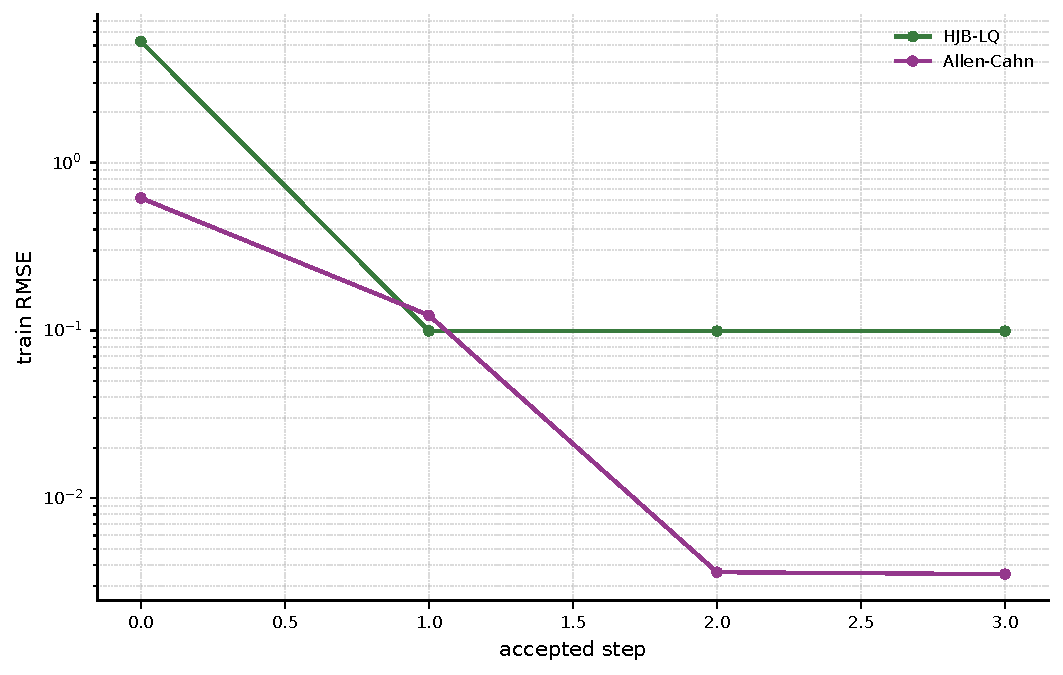
\includegraphics[height=0.42\textheight,width=\textwidth,keepaspectratio]{nonlinear-lm-residual}
        \caption{半线性方程 LM 残差下降}
      \end{figure}
    \end{column}
    \begin{column}{0.49\textwidth}
      \begin{figure}
        \centering
        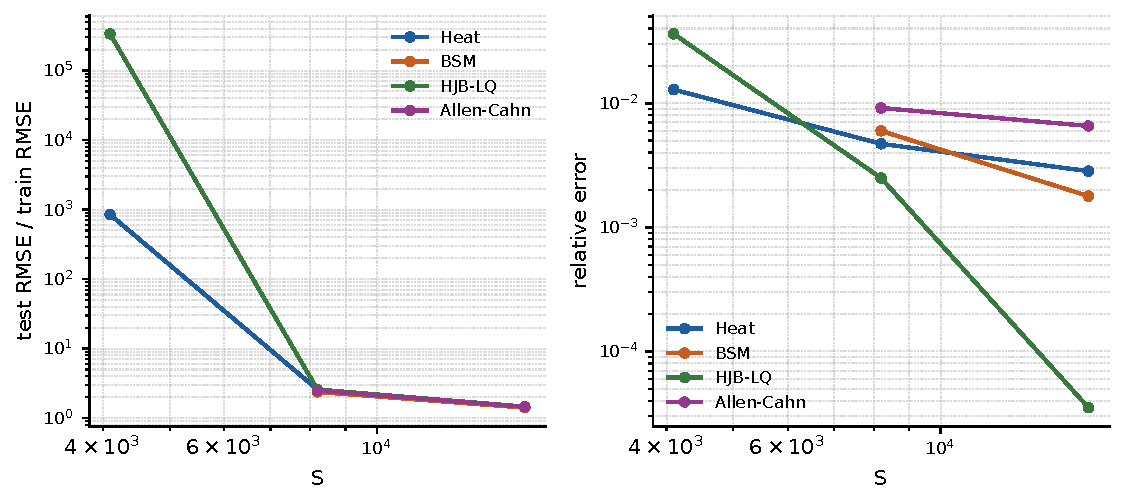
\includegraphics[height=0.42\textheight,width=\textwidth,keepaspectratio]{sample-size-generalization}
        \caption{样本数对泛化的影响}
      \end{figure}
    \end{column}
  \end{columns}

  \vspace{-0.05cm}
  \begin{block}{观察}
    小样本下可能出现训练残差很小但测试残差和初值误差较大的情况, 因此独立测试路径是必要的诊断指标.
  \end{block}
\end{frame}

\begin{frame}{维度扩展与方法对比}
  \begin{columns}[T,onlytextwidth]
    \begin{column}{0.50\textwidth}
      \begin{figure}
        \centering
        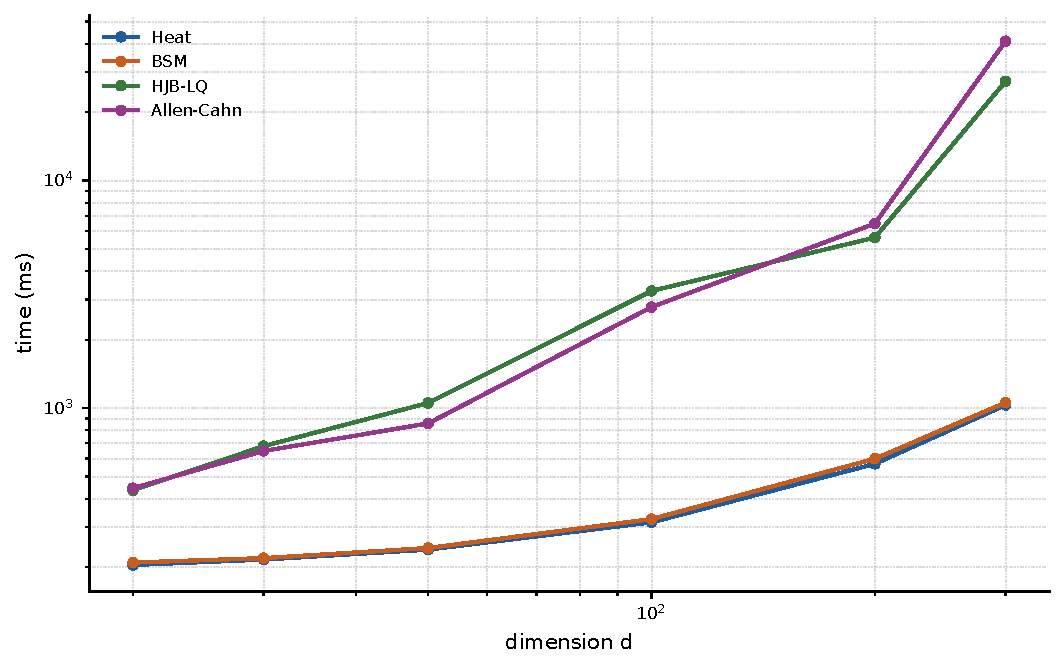
\includegraphics[width=\textwidth]{dimension-time-scaling}
        \caption{运行时间随维度变化}
      \end{figure}
    \end{column}
    \begin{column}{0.46\textwidth}
      \begin{table}
        \centering
        \scriptsize
        \begin{tabular}{llcc}
          \toprule
          方程 & 方法 & 时间 / s & 相对误差 \\
          \midrule
          HJB-LQ & RFM & 3.378 & 0.0035\% \\
          HJB-LQ & Deep BSDE & 15.221 & 0.077\% \\
          Allen-Cahn & RFM & 3.149 & 0.656\% \\
          Allen-Cahn & Deep BSDE & 29.192 & 0.116\% \\
          \bottomrule
        \end{tabular}
      \end{table}
      \begin{block}{对比结论}
        在本文实现和参数下, RFM 用更短时间得到接近参考值的初值. 精度优势依赖具体方程, Allen-Cahn 上 Deep BSDE 更精确但耗时更长.
      \end{block}
    \end{column}
  \end{columns}
\end{frame}

\section{总结展望}

\begin{frame}{总结与展望}
  \begin{block}{本文工作}
    \begin{itemize}
      \item 将高维抛物型 PDE 转化为 BSDE 路径匹配问题.
      \item 用固定内层随机特征近似 $Z_k$, 只训练 $y_0$ 和输出层参数 $\alpha$.
      \item 线性问题求解岭最小二乘, 半线性问题求解 LM 非线性最小二乘.
      \item 在四个 $100$ 维标准算例上取得接近参考值的初值.
    \end{itemize}
  \end{block}

  \begin{block}{后续方向}
    \begin{itemize}
      \item 分析采样误差, 时间离散误差和随机特征逼近误差的相对贡献.
      \item 改进特征尺度选择, 结构化随机特征和特征筛选, 缓解病态最小二乘.
      \item 对半线性问题引入无矩阵 LM/Gauss-Newton 或分块求解, 降低高维下显存和线性代数开销.
    \end{itemize}
  \end{block}
\end{frame}

\begin{frame}[plain]
  \begin{center}
    \vspace{1.1cm}
    {\Huge 谢谢各位老师!}

    \vspace{0.9cm}
    {\large 敬请批评指正}

    \vspace{1.1cm}
    
\includegraphics[height=1.15cm]{ustc-badge}
  \end{center}
\end{frame}

\end{document}
